\documentclass[a4paper,envcountsame,runningheads]{llncs}
\pdfmapfile{+cm-super-t1.map}
\usepackage[T1]{fontenc}
\usepackage[utf8]{inputenc}
\usepackage{amsmath,amssymb,booktabs,array,graphicx,tikz,placeins}
\usepackage[ruled,linesnumbered]{algorithm2e}
\usetikzlibrary{arrows.meta,positioning}
\usepackage[hidelinks,hypertexnames=false]{hyperref}
\hypersetup{pdftitle={LULA I: Rollback-Resilient Hash-Based Signatures with Cache-Accelerated Signing},pdfauthor={Luis Ángel Gonzalez},pdfsubject={LULA research family of hash-based signature schemes, Ring0 Labs, published by Lugel Labs},pdfkeywords={LULA, LULA I, hash-based signatures, rollback, cache}}
\usepackage[capitalise,noabbrev]{cleveref}
\pagestyle{plain}
\renewcommand{\figurename}{Figure}
\setlength{\emergencystretch}{2em}
\newcolumntype{P}[1]{>{\raggedright\arraybackslash}p{#1}}
\newcommand{\Hh}{\mathsf{SHA256}}
\newcommand{\Tr}{\mathsf{Trunc}_{16}}
\newcommand{\KG}{\mathsf{KeyGen}}
\newcommand{\Sign}{\mathsf{Sign}}
\newcommand{\Vf}{\mathsf{Verify}}
\newcommand{\CP}{\mathsf{CachePrepare}}
\newcommand{\AD}{\mathsf{ADRS}}
\newcommand{\Th}{\mathsf{Th}}
\newcommand{\BE}{\mathsf{BE}_{4}}
\newcommand{\bits}{\mathsf{bits}}
\newcommand{\Chain}{\mathsf{Chain}}
\newcommand{\Root}{\mathsf{Root}}
\newcommand{\Auth}{\mathsf{Auth}}
\newcommand{\Ctr}{\mathsf{FirstCounter}}
\newcommand{\Adv}{\mathsf{Adv}}
\newcommand{\eps}{\varepsilon}
\SetKw{Return}{return}
\SetKwInput{Input}{Input}
\SetKwInput{Output}{Output}
\begin{document}
\raggedbottom
\title{LULA I: Rollback-Resilient Hash-Based Signatures with Cache-Accelerated Signing}
\titlerunning{LULA I: Cache-Accelerated Hash-Based Signatures}
\author{Luis \'Angel Gonzalez}
\authorrunning{L.\,\'A. Gonzalez}
\institute{Ring0 Labs\\Published by Lugel Labs}
\maketitle
\thispagestyle{plain}
\begin{abstract}
LULA is Ring0 Labs' research family of hash-based signature schemes. This first paper presents LULA I, a deterministic signer accelerated by reusable caches. For successfully generated keys and honest prepared, restored or absent caches, we prove reference-signer agreement on termination and returned signature bytes. An atomic rollback simulation transfers an applicable reference bound without signing-query loss; the complete reference-signer bound remains open. Signatures are 5,720 bytes; cache payload is approximately 72 MiB. On one host, prepared-signing medians were 3.56--3.64 ms across three message lengths. Three individual first signatures after cache loss took 330.049--337.563 s.
\keywords{Hash-based signatures \and Rollback \and Caching \and WOTS+C \and FORS+C}
\end{abstract}

\section{Introduction}\label{sec:introduction}
LULA is Ring0 Labs' research family of hash-based signature schemes. This first paper presents LULA I and studies how honest cache restoration affects the signing function and its computation cost.

An adaptive adversary may obtain signatures from several executions of the same signer, each resumed from an older snapshot. The adversary retains the union of signatures published across these executions. A resource that appears unused after restoration may already have been exposed in another branch. Consequently, protecting a local consumption counter does not by itself protect a hash-based signing key against restoration.

The question studied here is whether mutable state can accelerate a hash-based signer without controlling which authorization resources it consumes. LULA I answers a restricted version constructively: its cache stores computations for a single deterministic reference signing function. Whenever signing terminates, the same message and key produce the same signature after an honest cache restoration, after cache deletion, or with caching disabled. Any unforgeability claim after restoration remains conditional on an applicable bound for the common reference signer.

The intended use objective is $2^{40}$ signing queries across all branches, conditional on a full reference-signer bound that has not yet been established. The FORS+C component analysis appears in \Cref{sec:operating}.

A large upper Merkle tree can be computed once and retained, while signing recomputes only smaller lower trees. Counters used to search for acceptable WOTS+C digests can also be prepared for message-independent child roots. Counter selection must be canonical: two counters for the same root can select different digests. Caching a counter without specifying its recomputation rule can therefore introduce the multiple-exposure problem that caching was intended to avoid.

Stateless hash-based signatures, their caches, and counter-based compression are established techniques. SPHINCS+ supplies the underlying FORS/hypertree architecture~\cite{sphincs}; SPHINCS+C supplies compressed component designs~\cite{sphincsc}; Gravity-SPHINCS already uses secret-key caching~\cite{gravity}. LULA I combines these components with canonical counters and a reusable top-tree cache.

Cache loss changes computation time even when signature bytes are preserved. The height-21 cached top tree requires billions of compressions to reconstruct. \Cref{sec:cost} derives this cost and summarizes selected latency observations. Output invariance and recovery cost are distinct properties of the mechanism.

\subsection{Our contributions}\label{sec:scope}

\begin{enumerate}
\item We specify one parameter set, its complete wire format, and its signature, cache, and work accounting (\Cref{sec:construction,sec:cache,sec:cost}).
\item We prove deterministic cache transparency, including termination equivalence, for successfully generated keys and honest cache states (\Cref{lem:transparent}).
\item We give a rollback-game simulation conditional on the common reference signer's security, and a counterexample to a general converse from frozen-state security (\Cref{thm:transfer,sec:frozen}).
\item We analyze canonical counter selection and the distinction between honest restoration and counter corruption (\Cref{sec:security}).
\item We derive cache, signing and verification costs and summarize their measured performance implications (\Cref{sec:cost}).
\end{enumerate}

The security result is a transfer theorem: rollback access preserves any applicable security bound for the common reference signing algorithm. It does not derive that reference bound from the underlying hash construction. The proof concerns honest snapshot restoration and atomic completed-call observations; edited cache contents, interrupted execution and leakage require different interfaces.

\Cref{sec:preliminaries} introduces the notation and rollback game. \Cref{sec:construction} specifies LULA I, and \Cref{sec:security} establishes correctness, cache transparency and the conditional rollback transfer. \Cref{sec:cache,sec:cost} describe the cache architecture, signature format and computational costs. Discussion and conclusions follow in \Cref{sec:limits,sec:conclusion}; \Cref{app:search} gives the asymptotic and counter-search analysis.

\subsection{Related work}\label{sec:related}
\paragraph{Stateful and stateless authorization.}
XMSS authenticates one-time keys with Merkle paths and requires that an index not be reused~\cite[Sections~4.1 and 4.1.9]{xmss}. SPHINCS+ uses a few-time component selected by a message digest and certifies it through a hypertree~\cite{sphincs}. SLH-DSA standardizes this architecture with specified hash functions and parameters~\cite{fips205}. LULA I follows the stateless architecture, rather than attempting to make a consumption index survive restoration.

\paragraph{Compressed components and variable layers.}
SPHINCS+C searches for digest subsets that permit shorter WOTS and FORS evidence~\cite{sphincsc}. A fixed digit sum replaces a conventional checksum in the WOTS+C component considered here. Kudinov and Nick analyze alternative component choices~\cite[Sections 5 and 13]{kn}. Qin, Sun, and Zheng consider varying heights and chain lengths across layers~\cite{variable}. LULA I uses different heights and widths at different layers; these choices define the concrete signing function whose cache behavior we study.

\paragraph{Caching and reset attacks.}
Gravity-SPHINCS demonstrates that caching can change signing cost and the parameter tradeoff~\cite{gravity}. Ristenpart and Yilek analyze virtual-machine reset vulnerabilities and hedging against randomness failures~\cite{reset}. Our deterministic signer consumes no online random-generator state. It therefore avoids dependence on a restored generator, conditional on the security of its message-dependent derivation. This does not establish that determinism alone implies security.

\paragraph{Limited-use parameter sets.}
NIST SP 800-230's initial public draft proposes additional SLH-DSA parameter sets with a $2^{24}$ lifetime signature limit and permits hypertree caching~\cite[Table~1 and Section~3]{sp800230}. Its 3,856-byte SHA2-128-24 signatures illustrate why query limits must accompany size comparisons. Fluhrer and Dang analyze FORS coverage using an occupancy model~\cite[Section~5]{fluhrer}; \Cref{sec:operating} states the additional modeling assumptions used for LULA I.

\paragraph{Positioning.}
The third-party Go implementation uses the smallest valid WOTS+C counter~\cite{hashsiggo}. LULA I likewise requires canonical selection so that cache reconstruction returns the same counter as preparation. Its contribution is the specified integration and the conditional rollback-transfer argument, rather than a new hardness assumption or a general security property of stateless signatures.

\section{Preliminaries}\label{sec:preliminaries}
\subsection{Notation}\label{sec:notation}
All hash nodes are $n=16$ bytes. $\Hh$ produces 32 bytes; $\Tr$ selects its first 16 bytes. Concatenation is denoted by $\|$. All integer fields use big-endian byte order. $\BE(c)$ encodes a 32-bit unsigned integer. $\bits(D,s,r)$ reads $r$ bits starting at zero-based bit offset $s$, most-significant bit first. Messages are finite byte strings $M$ with length $L$.

For a binary Merkle tree of height $h$, a path contains $h$ sibling nodes, from the leaf upward. At each level the index parity determines the left/right order. The address includes the height and parent index. A subtree is represented in level-major order: leaves first, then each successive level, ending at the root.

The hypertree has $d$ layers numbered $j=0,\ldots,d-1$ from bottom to top. Layer $j$ has height $h_j$, width $w_j=2^{b_j}$, and $\ell_j=128/b_j$ WOTS chains. The evaluated set has no forced-zero WOTS digits. Its required digit sum is $S_j=\ell_j(w_j-1)/2$. Define $h=\sum_j h_j$ and $s_j=\sum_{i<j}h_i$. For an $h$-bit index $I$, the leaf and tree indices are
\begin{equation}\label{eq:route}
 q_j=(I\mathbin{\gg}s_j)\bmod 2^{h_j},\qquad
 t_j=I\mathbin{\gg}(s_j+h_j).
\end{equation}
The FORS+C digest addresses $k$ trees of height $a$ but forces the last index to zero. Only $k'=k-1$ trees are instantiated and transmitted. This omission is part of the compressed construction; no secret from an omitted tree is serialized.

\subsection{Atomic chosen-message rollback game}\label{sec:game}
Let $\Pi=(\KG,\Sign,\Vf)$ be a signature scheme whose key-generation algorithm $\KG$ returns a public key $pk$, a secret key $sk$, and initial mutable state $\mu_0$. A challenger gives $pk$ to an adversary $\mathcal A$ and maintains a current state, a handle-indexed snapshot store, and a permanent message set $\mathcal Q$. The initial snapshot has handle 0; subsequent snapshots receive sequential integer labels that disclose no state contents. The following commands are allowed:
\begin{itemize}
\item $\mathsf{Sign}(M)$ returns $\sigma$ and updates the current state atomically; it adds $M$ to $\mathcal Q$.
\item $\mathsf{Snapshot}()$ stores the complete current restorable state and returns an opaque handle.
\item $\mathsf{Restore}(u)$ restores a previously stored snapshot. It does not remove messages from $\mathcal Q$ or erase the adversary's observations.
\end{itemize}
The adversary may restore the initial snapshot or snapshots between any two completed signing calls, branch repeatedly, and choose its next message adaptively. State contents remain secret. Restoration installs an honest earlier state of the same key and parameter set; arbitrary edited bytes are not a restoration operation in this game.

At most $Q$ signing queries are counted across all branches. The adversary also has computational budget $T$ and, in a random-oracle formulation, at most $q_H$ adversarial hash-oracle queries. The time budget counts local adversary and simulator computation; the honest signing oracle's internal work is accounted for separately in \Cref{sec:cost}. Snapshot and restoration commands are finite and bounded by the adversary's total resources, but no fixed security-critical restoration limit is imposed. A fresh-message forgery wins when
\begin{equation}\label{eq:win}
 \Vf(pk,M^*,\sigma^*)=1\quad\text{and}\quad M^*\notin\mathcal Q.
\end{equation}
Define $\Adv^{\mathrm{euf\text{-}cma\text{-}rb}}_{\Pi}(\mathcal A)$ as the probability of this event over key generation, adversarial coins, and any explicitly modeled hash or signing randomness. The definition is parameterized by $(Q,T,q_H)$; fixing $Q$ alone does not specify a concrete security level.

Ordinary existential unforgeability under chosen-message attacks (EUF-CMA) removes snapshot and restoration commands. It uses the same permanent freshness set. We study existential unforgeability, not strong unforgeability: another signature on a queried message is not a winning forgery.

\subsection{Randomness and observation model}
In a restored-randomness model, generator state is part of the snapshot. In a fresh-entropy model, new independent coins remain available after restoration. LULA I's implemented signer is deterministic given $(sk,M)$ and does not call either generator, so both models induce the same outputs. Key generation requires securely sampled secret material.

The game omits elapsed times, crash behavior, partial signatures, and access to the cache bytes. It therefore proves no timing noninterference or leakage guarantee. Mid-call restoration is excluded by atomicity. A nonterminating signing request prevents that experiment from reaching a winning completion. A real implementation that publishes partial work, resumes corrupted execution frames, or reveals timing information needs a stronger model.

\section{LULA I construction}\label{sec:construction}
\subsection{Parameters and key material}
\Cref{tab:params} fixes the evaluated parameter set; \Cref{sec:memorytradeoff} also gives an unevaluated height illustration. The evaluated digest uses $ka+h=203$ of the 256 output bits, including nine forced-zero bits. The public key is $PK.seed\|PK.root$ (32 bytes). The stored master seed is $SK.seed\|SK.prf\|PK.seed$ (48 bytes); each component is 16 bytes. The public root is also retained by the signer. Expanded context and allocations are additional memory, not additional transmitted key fields.

\begin{table}[t]
\caption{The single evaluated LULA I parameter set. The last column identifies prepared layers; it is not an authorization counter.}\label{tab:params}
\centering\small
\begin{tabular}{lrrrrrl}\toprule
Component & $h_j$ & $b_j$ & $w_j$ & $\ell_j$ & $S_j$ & Cache\\\midrule
Layers 0--3, each &5&4&16&32&240&No\\
Layer 4 &21&8&256&16&2040&Yes\\\bottomrule
\end{tabular}

\smallskip
\begin{tabular}{lr@{\quad}lr}\toprule
Node bytes $n$&16&Total height $h$&41\\
FORS digest trees $k$&18&FORS height $a$&9\\
Transmitted trees $k'$&17&Hypertree layers $d$&5\\\bottomrule
\end{tabular}
\end{table}

\subsection{Addresses and hashes}\label{sec:hash}
An address is exactly 22 bytes:
\[
 \AD=\mathsf{layer}_1\|\mathsf{tree}_8\|\mathsf{type}_1
       \|\mathsf{keypair}_4\|\mathsf{word2}_4\|\mathsf{word3}_4.
\]
Subscripts give field sizes in bytes. Types 0--7 denote WOTS chain, WOTS public-key compression, hypertree node, FORS node, FORS-root compression, WOTS-secret derivation, FORS-secret derivation, and WOTS+C message digest, respectively. Word 2 is a chain index or tree height; word 3 is a chain position or node index. Unused fields are zero. These types separate the implemented domains; they do not imply that arbitrary uses of SHA-256 satisfy all required cryptographic assumptions.

For byte string $X$, the implemented tweakable function is
\begin{equation}\label{eq:th}
 \Th(A,X)=\Tr\bigl(\Hh(PK.seed\|0^{48\,\mathrm{bytes}}\|A\|X)\bigr).
\end{equation}
The leaf function is $F(A,x)=\Th(A,x)$ and the binary node function is $H(A,x,y)=\Th(A,x\|y)$. Secret derivation uses $\mathsf{PRF}(A)=\Th(A,SK.seed)$. SHA-256's compression state after the first 64-byte prefix is prepared once per context. No nonstandard compression padding is introduced.

The message functions are
\begin{align}\label{eq:message}
 R(M)&=\Tr\bigl(\Hh(SK.prf\|PK.seed\|M)\bigr),\nonumber\\
 U(M)&=\Hh(R(M)\|PK.seed\|PK.root\|M),\\
 D_c(M)&=\Hh(U(M)\|\BE(c)\|PK.seed).\nonumber
\end{align}
The signer selects the smallest $c\in\{0,\ldots,2^{32}-1\}$ for which $\bits(D_c,153,9)=0$. The first 153 bits select 17 FORS indices; bits 162--202 select $I$. Verification recomputes these values using transmitted $R$ and $c$, rather than checking that $R$ was secretly derived. Consequently, an unforgeability argument must cover adversarial choices of both fields.

These functions differ from standardized SLH-DSA's HMAC-based message randomizer, message expansion, and external context interface~\cite[Sections~10.2, 10.3, and 11.2]{fips205}. LULA I is not SLH-DSA conformant. Its raw-message interface provides no standardized application-context or prehash wrapper.

\subsection{WOTS+C keys}
For address $(j,t,q)$ and a 16-byte value $V$, let
\[
 E_c(V)=\Th(\AD(j,t,7,q,0,0),V\|\BE(c)).
\]
Read $E_c(V)$ as $\ell_j$ base-$w_j$ digits $e_0,\ldots,e_{\ell_j-1}$. A counter is accepted when $\sum_i e_i=S_j$. $\Ctr(j,t,q,V)$ returns the smallest accepted counter. The secret chain start is
\[
 x_i=\mathsf{PRF}(\AD(j,t,5,q,i,0)).
\]
To advance from position $u$ by $v$ steps, apply $F(\AD(j,t,0,q,i,p),\cdot)$ successively for $p=u,\ldots,u+v-1$. The public key is the type-1 compression of all endpoints at position $w_j-1$. A signature on $V$ contains $c$ and the $\ell_j$ chain values at positions $e_i$. Verification completes each chain and compresses the endpoints.

Layer-tree leaves are these WOTS public keys. A type-2 address identifies each Merkle node by $(j,t,\text{height},\text{index})$. The child value signed at layer 0 is the FORS public key associated with $(t_0,q_0)$. For layer $j>0$, it is the root of subtree $(j-1,\,t_j2^{h_j}+q_j)$. Both values are fixed by the key and address, independently of the message that routes through them.

\subsection{FORS+C component}
For tree $r\in\{0,\ldots,16\}$ and leaf $i<512$, define the global index $g=512r+i$. The secret is the type-6 PRF at $(0,t_0,q_0,g)$; its leaf image is the type-3 hash at height zero and index $g$. At height $v$, the address index is $r2^{a-v}+i_v$, where $i_v$ is the local index at that level. A FORS signature reveals one selected secret and its nine siblings per tree. A type-4 compression of the 17 reconstructed roots gives $V_0$.

The implementation instantiates only the 17 real trees; no implicit secret is transmitted for the omitted tree. Both signing and verification enforce the zero condition on the eighteenth index.

\subsection{Key generation and cache preparation}
\Cref{alg:kg,alg:prepare} define key generation from a securely sampled seed and cache preparation. LULA I prepares one height-21 top subtree and one canonical counter for each of its $2^{21}$ leaves. Preparing a counter requires the corresponding height-5 child root.

\begin{algorithm}[t]
\caption{LULA I KeyGen}\label{alg:kg}
\Input{Parameters in \Cref{tab:params}; securely sampled 48-byte seed $s$}
\Output{$(pk,sk,C)$}
Split $s$ into $(SK.seed,SK.prf,PK.seed)$\;
Initialize the seed-derived hash context $\mathsf{ctx}$ from $(SK.seed,SK.prf,PK.seed)$, including the SHA-256 prefix state\;
$C\leftarrow\CP(\mathsf{ctx})$ using \Cref{alg:prepare}\;
$PK.root\leftarrow C.\mathsf{topTree}.\mathsf{root}$\;
$pk\leftarrow PK.seed\|PK.root$\;
\Return{$(pk,(s,PK.root),C)$}\;
\end{algorithm}

\begin{algorithm}[t]
\caption{LULA I CachePrepare}\label{alg:prepare}
\Input{Seed-derived hash context $\mathsf{ctx}$ and fixed parameters}
\Output{Top-tree nodes and canonical counters}
\For{$q=0,\ldots,2^{21}-1$}{
 $y_q\leftarrow\mathsf{WotsPK}(4,0,q)$\;
 $V_q\leftarrow\Root(\mathsf{Subtree}(3,q))$\;
 $c_q\leftarrow\Ctr(4,0,q,V_q)$\;
}
$T\leftarrow\mathsf{MerkleBuild}(4,0,y_0,\ldots,y_{2^{21}-1})$\;
\Return{$C=(T,(c_q)_{q<2^{21}})$}\;
\end{algorithm}

\subsection{Signing and public verification}
\Cref{alg:sign,alg:verify} specify the transmitted object, including every counter. Neither algorithm consults a consumption index. An honest cache entry changes which computations are repeated; it does not change their outputs.

\begin{algorithm}[t]
\caption{LULA I Sign}\label{alg:sign}
\Input{$(sk,PK.root,C,M)$}
\Output{Serialized signature $\sigma$}
Compute $R,U$ from \Cref{eq:message}\;
$c_F\leftarrow$ smallest counter with $\bits(D_{c_F},153,9)=0$\;
Extract $i_0,\ldots,i_{16}$ and $I$ from $D_{c_F}$\;
Derive $(t_0,q_0)$ from \Cref{eq:route}\;
$(\sigma_F,V)\leftarrow\mathsf{ForsSign}(t_0,q_0,(i_r)_r)$\;
$\sigma\leftarrow R\|\BE(c_F)\|\sigma_F$\;
Let $x_i^{(j)}$ denote the secret chain starts at leaf $(j,t_j,q_j)$, as defined in the WOTS+C section\;
\For{$j=0,\ldots,4$}{
 Derive $(t_j,q_j)$ from \Cref{eq:route}\;
 Obtain $(c,T)$ by \Cref{alg:restore}\;
 $e\leftarrow$ digits of $E_c(V)$\;
 $W\leftarrow(\Chain(x_i^{(j)},0,e_i))_{i<\ell_j}$\;
 $\sigma\leftarrow\sigma\|\BE(c)\|W\|\Auth(T,q_j)$\;
 $V\leftarrow\Root(T)$\;
}
\Return{$\sigma$}\;
\end{algorithm}

\begin{algorithm}[t]
\caption{LULA I Verify}\label{alg:verify}
\Input{$(pk,M,\sigma)$}
\Output{Boolean}
Reject unless $|pk|=32$ and $|\sigma|=5720$\;
Parse fields in the order of \Cref{tab:wire}\;
Recompute $U,D_{c_F}$ from transmitted $R,c_F$ and $(pk,M)$\;
Reject unless $\bits(D_{c_F},153,9)=0$\;
Extract FORS indices and $I$; derive $(t_0,q_0)$\;
$V\leftarrow\mathsf{ForsPKFromSig}(t_0,q_0,(i_r)_r,\sigma_F)$\;
\For{$j=0,\ldots,4$}{
 Derive $(t_j,q_j)$; read the layer counter $c_j$\;
 $e\leftarrow$ digits of $E_{c_j}(V)$\;
 Reject unless $\sum_i e_i=S_j$\;
 Reconstruct the WOTS public key $P_j$ by completing each chain\;
 $V\leftarrow\mathsf{RootFromPath}(j,t_j,q_j,P_j,\mathsf{path}_j)$\;
}
\Return{$V=PK.root$}\;
\end{algorithm}



\begin{algorithm}[t]
\caption{LULA I CacheRestore: cache lookup and cache-miss recomputation}\label{alg:restore}
\Input{Layer $j$, route $(t,q)$, current child value $V$, honest cache $C$}
\Output{Counter $c$ and subtree $T$}
\eIf{$j=4$ and the complete top-layer cache is present}{
 $T\leftarrow C.\mathsf{topTree}$; $c\leftarrow C.\mathsf{counters}[q]$\;
 \If{$c$ does not satisfy the digit-sum predicate for $V$}{
 $c\leftarrow\Ctr(j,t,q,V)$\;
 }
}{
 $c\leftarrow\Ctr(j,t,q,V)$\;
 $T\leftarrow\mathsf{BuildSubtree}(j,t)$\;
}
\Return{$(c,T)$}\;
\end{algorithm}

Restoration installs an honest copy of the prepared cache. \Cref{alg:restore} specifies lookup and recomputation; it does not authenticate arbitrary edited cache contents.

\section{Correctness and security}\label{sec:security}
\subsection{Correctness}\label{sec:correctness}
\begin{lemma}[Chain and tree reconstruction]\label{lem:correct}
For a successfully generated key and terminating counter searches, a signature produced with honest cache contents is accepted by the verifier.
\end{lemma}
\begin{proof}
Completing a chain from its signed position $e_i$ applies the remaining $w_j-1-e_i$ addressed hashes, yielding the same endpoint used in its public key. Public-key compression therefore reconstructs the corresponding leaf. Each authentication path then reconstructs its subtree root with the same addressed left/right ordering. FORS reconstruction begins with the revealed secret and reconstructs its selected leaf and root in each of the 17 trees. Its root compression equals the value signed at layer 0. Induction over the five hypertree layers gives the top-tree root fixed at key generation. The digest predicates hold by the counter searches. The serialized length equals the parser's required length by \Cref{eq:size}.\qed
\end{proof}

Counter searches are partial computations over a 32-bit counter space. An accepted counter is not assumed to exist for every input. \Cref{lem:correct} is therefore conditional on termination; counter exhaustion is outside the successful-return behavior specified here.

\subsection{Reference-signer security}
The security of the reference signer is a premise of the rollback transfer. The mechanism does not establish primitive or composition bounds for its secret derivations, message randomizer, FORS disclosure, WOTS+C substitutions or Merkle compressions. An applicable reference bound must cover the exact signing function and the public verifier, including adversarial choices of the transmitted randomizer and counters.

The transfer proof compares the public signing interfaces and does not depend on a particular hash idealization. Its signing-query and adversarial hash-query accounting excludes honest oracle-internal work, which changes with cache availability. The result concerns preservation of a reference bound under the declared restoration interface.

\subsection{Constant-sum chains and repeated certification}
For two accepted digit vectors $e,e'$ with the same sum $S_j$, componentwise domination $e'_i\ge e_i$ for all $i$ implies $e'=e$. Thus one WOTS+C exposure cannot reach a different accepted digit vector solely by advancing every chain. This antichain fact explains the target-sum predicate, but leaves digest collisions, inversions, multi-target attacks, and certification composition to the cryptographic proof.

When two distinct accepted vectors are exposed at the same address, their coordinatewise minima can have sum below $S_j$. A new target vector can then dominate those minima while still having sum $S_j$. Canonical counter selection prevents this particular second-vector exposure during honest repeated certification. A public verifier checks acceptance of a counter, not its minimality; signer-side canonicality is therefore a security dependency.

\subsection{Restoration and cache corruption}
Arbitrary writes to cache nodes or counters are fault attacks. \Cref{alg:restore} recomputes a rejected counter, but accepts an alternative valid counter without testing minimality. A miniature instance yields a different accepted signature on the same message after such a write. This is not a fresh-message forgery, but it disproves transparency under arbitrary counter corruption. Adjacent cached layers additionally require integrity protection when their roots become values signed by upper keys.

\subsection{Cache transparency and rollback transfer}\label{sec:rollback}
Let $\Sign^\circ(sk,M)$ be the reference algorithm with every layer recomputed and all searches starting at zero. Let $\mathcal C(sk)$ contain either the complete honest top-layer cache or its absent representation. For LULA I, these are the supported cache regimes; restoring an older prepared cache yields the same entries because signing does not modify them.

\begin{lemma}[Deterministic cache transparency]\label{lem:transparent}
For each successfully generated key, message $M$, and $C\in\mathcal C(sk)$, signing with $C$ terminates if and only if the reference signing request terminates. Whenever they terminate,
\[
 \Sign(sk,C,M)=\Sign^\circ(sk,M).
\]
Deleting any whole configured cache layer has the same property in parameter sets whose cached layers form a top segment and whose remaining entries are honest.
\end{lemma}
\begin{proof}
The message functions and selected route do not read the cache. The FORS computation is unchanged. At an uncached layer, the reference computation is performed directly. At a cached layer, the stored subtree is exactly its deterministic seed-derived subtree. Its child value equals the root of the referenced child subtree, whether that root is recomputed or honestly cached. The stored counter is the smallest accepted counter for that value and address, exactly as in the reference search. Successful preparation proves that this counter exists, so the corresponding reference search terminates. The remaining searches are identical in both executions. Thus termination agrees, and chain signatures and paths match whenever both executions terminate. Induction over the layers yields equality of all output fields.\qed
\end{proof}

\begin{theorem}[Rollback-security transfer]\label{thm:transfer}
Suppose a deterministic signer satisfies \Cref{lem:transparent}, including termination equivalence, for every honestly reachable and restorable state, shares its public key and verifier with $\Pi^\circ$, and emits only completed signatures. A nonterminating signing request produces no further public response in either game; explicit failure responses, crashes, and timing observations require their own shared-oracle semantics. For every atomic rollback adversary $\mathcal A$ making at most $Q$ signing queries there is an ordinary EUF-CMA adversary $\mathcal B$ making the same number of queries such that
\[
 \Adv^{\mathrm{euf\text{-}cma\text{-}rb}}_\Pi(\mathcal A)
 =\Adv^{\mathrm{euf\text{-}cma}}_{\Pi^\circ}(\mathcal B).
\]
The simulator adds no adversarial hash-oracle queries and no probability loss. Honest signing-oracle work can differ between cache regimes and is not included in this query-preservation statement. Using sequential integer handles and direct-index membership checks, its bookkeeping requires a constant number of word-RAM operations per command, in addition to running $\mathcal A$. Handle encodings and bit-level costs depend on the number of snapshots.
\end{theorem}
\begin{proof}
$\mathcal B$ forwards every signing query to its reference signing oracle. It returns the next sequential integer handle for each snapshot and checks the range of restoration handles, without changing any cryptographic state. Termination equivalence preserves whether each signing request returns a response. By deterministic transparency, every returned signature is exactly the signature that $\mathcal A$ would receive after its selected history. Both games maintain the same permanent set of queried messages. Coupling the key, adversarial randomness, and hash interface therefore gives identical public transcripts and the same winning event. The bookkeeping uses no hash query.\qed
\end{proof}

\paragraph{Security consequence.}
The proof of \Cref{thm:transfer} is a transcript simulation for the stated atomic interface. If the exact reference signer has bound $\eps(Q,T,q_H)$, the rollback signer inherits that bound with the simulator's time overhead. No concrete $\eps$ for the full instantiation is established here. Rollback resilience here means this conditional transfer together with the proved equality of the signing function under honest restoration.

In LULA I, the construction-specific condition for the transfer theorem is deterministic cache transparency. LULA I has no mutable authorization index, and its cache is read-only during signing (\Cref{sec:construction,sec:cache}). A cache that selects a history-dependent counter can violate transparency: the cache-corruption example returns a different accepted chain vector at the same address (\Cref{sec:security}). The theorem therefore separates that mechanism-level condition from the unresolved security of the common reference signer.

State need not consist exclusively of deterministic key-derived bytes. A diagnostic counter or random eviction policy can be harmless if it preserves termination behavior and returned signatures in the declared interface. For randomized reference signers, equality of separate marginal distributions at each frozen state is insufficient when restored randomness creates correlations across calls; a joint transcript coupling is required.

\subsection{Frozen-state security and adaptive rollback}\label{sec:frozen}
Restoring one snapshot before every query gives an adversary access to its frozen signing function. Hence rollback security implies the appropriate frozen-state security, after charging the queries used to reach that state and preserving freshness across the reaching history. It does not follow that security of every frozen function implies security of an adaptive tree of branches.

The following generic counterexample makes the missing implication explicit. Take any secure stateless signature scheme with fixed-length secret key $sk$. Sample an independent uniform pad $x$ of that length and set $y=x\oplus sk$. The initial state signs normally and chooses an absorbing branch $b\in\{0,1\}$ according to a public bit of the first message. Subsequent signatures contain the normal signature and share $x$ if $b=0$, or $y$ if $b=1$; verification ignores that share. \Cref{fig:branches} shows why the permanent adversarial transcript combines branches.

\begin{figure}[!htbp]
\centering
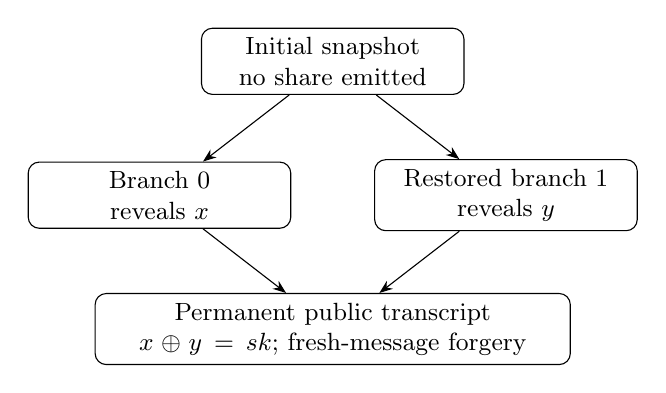
\begin{tikzpicture}[>=Stealth,
 b/.style={draw,rounded corners,align=center,text width=31mm,font=\small}]
\node[b] (snap) at (0,0) {Initial snapshot\\no share emitted};
\node[b] (a) at (-2.2,-1.7) {Branch 0\\reveals $x$};
\node[b] (bb) at (2.2,-1.7) {Restored branch 1\\reveals $y$};
\node[b,text width=58mm] (union) at (0,-3.4) {Permanent public transcript\\$x\oplus y=sk$; fresh-message forgery};
\draw[->] (snap)--(a);\draw[->] (snap)--(bb);
\draw[->] (a)--(union);\draw[->] (bb)--(union);
\end{tikzpicture}
\caption{A counterexample to the converse frozen-state implication. Each branch reveals one share that is individually independent of the secret key, but restoration does not erase the adversary's earlier observations. LULA I's honest caches avoid this mechanism by preserving one signing function.}\label{fig:branches}
\end{figure}

Each frozen initial signer is the base signer without a share. Each frozen absorbing signer reveals only one share, which is independent of $sk$ and can be simulated. A sequential path reveals at most one share. An adversary can instead snapshot the initial state, enter branch 0 and obtain $x$, restore, enter branch 1 and obtain $y$, recover $sk=x\oplus y$, and sign a fresh message. This is a conditional cryptographic counterexample built from any secure base scheme. This counterexample does not attack LULA I, whose honest caches preserve one common function.

\subsection{Signing-query objective and FORS coverage}\label{sec:operating}
We consider a use objective of $2^{40}$ signing queries across restored branches. It is conditional on the unresolved full reference-signer bound, rather than a certified signing capacity.

The model considers a generic classical FORS coverage attack, following the occupancy analysis of Fluhrer and Dang~\cite[Section~5, Equation~(1)]{fluhrer}. It assumes independent uniform address and tree-index selections. For LULA I, with $\rho=2^{-41}$, $r=1-2^{-9}$ and $N$ exposures at one address, coverage of the 17 real trees has probability $(1-r^N)^{17}$. A raw candidate must also satisfy the nine-bit zero condition. Expanding the power gives
\[
 p_{\mathrm{raw}}=2^{-9}\sum_{j=0}^{17}(-1)^j\binom{17}{j}\,\mathbb E[r^{jN}].
\]
For Binomial occupancy, $N\sim\mathrm{Bin}(q_{\mathrm{sig}},\rho)$ and $\mathbb E[r^{jN}]=(1-\rho+\rho r^j)^{q_{\mathrm{sig}}}$. The Poisson approximation uses $\lambda=q_{\mathrm{sig}}\rho$ and $\mathbb E[r^{jN}]=\exp(\lambda(r^j-1))$. Both evaluations agree at the displayed precision for LULA I.

\begin{table}[t]
\caption{Classical FORS+C coverage-model exponents per raw digest candidate for the fixed LULA I parameters. Independent uniform selections are assumed. These component values are not full-signature security bounds.}\label{tab:security-model}
\centering\small
\begin{tabular}{lr}\toprule
Signing queries & $-\log_2 p_{\mathrm{raw}}$\\\midrule
$2^{38}$ &143.3\\
$2^{40}$ &132.6\\
$2^{41}$ &125.9\\\bottomrule
\end{tabular}
\end{table}

At $2^{40}$ queries, 132.6 is a per-candidate FORS+C exponent, not a 128-bit bound for the complete signer. The calculation does not establish the selection distribution of the deterministic signer, control adaptive forged randomizers and counters, or close the hypertree and primitive reductions. Additional signing queries reduce the component exponent; no certified threshold follows from this model alone.

\FloatBarrier

\section{Cache-accelerated signing}\label{sec:cache}
\Cref{fig:dependency} separates the source of authorization from its accelerated computations. The secret seed defines chain starts and FORS secrets; public addresses define their domains. The cache supplies previously computed nodes and counters. It supplies no trusted record of previously signed messages.

\begin{figure}[!htbp]
\centering
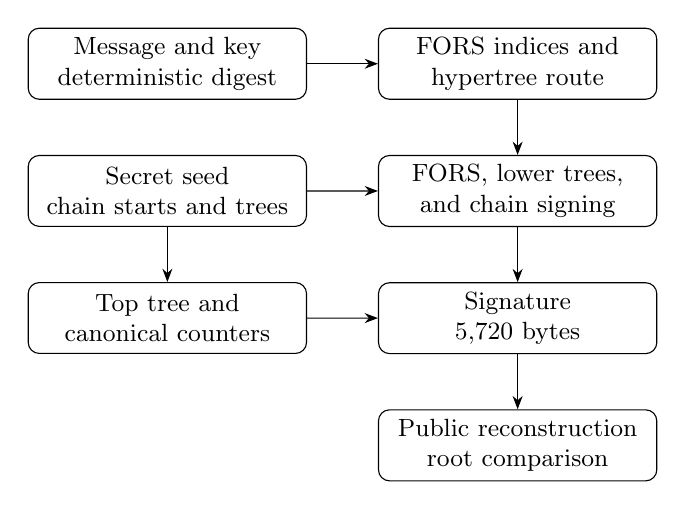
\begin{tikzpicture}[>=Stealth,node distance=7mm,
 box/.style={draw,rounded corners,align=center,font=\small,text width=33mm,minimum height=9mm}]
\node[box] (m) {Message and key\\deterministic digest};
\node[box,right=9mm of m] (route) {FORS indices and\\hypertree route};
\node[box,below=of m] (sk) {Secret seed\\chain starts and trees};
\node[box,below=of route] (online) {FORS, lower trees,\\and chain signing};
\node[box,below=of sk] (cache) {Top tree and\\canonical counters};
\node[box,below=of online] (sig) {Signature\\5,720 bytes};
\node[box,below=of sig] (vf) {Public reconstruction\\root comparison};
\draw[->] (m)--(route);\draw[->] (route)--(online);
\draw[->] (sk)--(online);\draw[->] (sk)--(cache);
\draw[->] (online)--(sig);\draw[->] (cache)--(sig);
\draw[->] (sig)--(vf);
\end{tikzpicture}
\caption{LULA I's dependency graph. Authorization follows the secret-derived objects and public verification. The cache accelerates fixed computations; removing the honest cache preserves signature bytes whenever signing terminates, but adds top-tree reconstruction and search.}\label{fig:dependency}
\end{figure}

The top cache contains $(2^{22}-1)$ nodes and $2^{21}$ counters. Its payload is exactly
\begin{equation}\label{eq:cache}
 C_{\mathrm{bytes}}=16(2^{22}-1)+4\cdot2^{21}
 =75{,}497{,}456\ \mathrm{bytes}.
\end{equation}
This is $72$ MiB minus 16 bytes. It excludes allocation headers, spare vector capacity, context and temporary preparation buffers; these are distinct from the cache payload.

Cache age does not enter the signing function: an older honest prepared snapshot contains the same nodes and canonical counters. A seed-only backup permits reconstruction but retains none of its computational acceleration. Without the top-layer cache, each signature recomputes that tree; signing does not itself retain a replacement cache.

\subsection{Less cache memory and the security claim}\label{sec:memorytradeoff}
The payload comprises $64$ MiB minus 16 bytes of tree nodes and $8$ MiB of counters. With the evaluated parameters unchanged, omitting the retained top cache preserves the 5,720-byte signatures, the reference signing function and its conditional security transfer. The cost is top-tree reconstruction and counter search on each signature. It does not eliminate working memory: uncached signing still materializes the temporary tree. The evaluated implementation supports a complete or absent top cache; intermediate cache policies are not implemented or measured here.

Reducing memory by changing parameters is a different choice. At fixed node and counter widths, a top tree of height $h_4$ has payload $36\cdot2^{h_4}-16$ bytes. As an analytical illustration, lowering $h_4$ from 21 to 20 while retaining four height-5 lower layers gives $37{,}748{,}720$ bytes ($36$ MiB minus 16 bytes), 5,704-byte signatures and total height 40. At $2^{40}$ signing queries, the same independent-selection FORS+C model gives a per-candidate exponent of 125.9 instead of 132.6. This is an unevaluated component calculation, not a full-security bound. Reallocating the removed height to another layer changes the work balance and requires a separate parameter analysis.



\section{Signature format, computational cost, and performance}\label{sec:cost}

\subsection{Exact wire format}
\Cref{tab:wire} gives every transmitted field in order. The parameter set is fixed externally and no parameter identifier is included in the signature. This is acceptable for a fixed-parameter interface but requires an explicit protocol identifier when integrating multiple schemes.

\begin{table}[t]
\caption{LULA I signature serialization. Offsets are zero based; counters are 32-bit big-endian integers. No message, public key, or padding is included in the signature.}\label{tab:wire}
\centering\small
\begin{tabular}{P{49mm}rr}\toprule
Field & Offset & Bytes\\\midrule
Randomizer $R$ &0&16\\
FORS+C counter $c_F$ &16&4\\
17 FORS secrets and nine-node paths &20&2720\\
Layer 0: counter, 32 values, 5 siblings &2740&596\\
Layer 1: counter, 32 values, 5 siblings &3336&596\\
Layer 2: counter, 32 values, 5 siblings &3932&596\\
Layer 3: counter, 32 values, 5 siblings &4528&596\\
Layer 4: counter, 16 values, 21 siblings &5124&596\\\midrule
Total &&5720\\\bottomrule
\end{tabular}
\end{table}

The size follows directly from the loops in \Cref{alg:sign}:
\begin{align}\label{eq:size}
 |\sigma|&=16+4+16\cdot17(9+1)
      +\sum_{j=0}^{4}(4+16\ell_j+16h_j)\nonumber\\
 &=16+4+2720+5\cdot596=5720\ \mathrm{bytes}.
\end{align}
Each layer happens to occupy 596 bytes for this set: the top layer trades 16 fewer chain values for 16 more path nodes. This equality does not hold for arbitrary parameter sets.

\subsection{Verification complexity}
Let $b(x)=\lceil(x+9)/64\rceil$ be the number of SHA-256 blocks for an $x$-byte suffix after a prepared 64-byte prefix. A WOTS public-key compression costs $b(22+16\ell_j)$ additional compressions. Chain completion costs $\ell_j(w_j-1)-S_j$, which is constant for accepted digit vectors.

For a 32-byte message, verification requires 3,265 SHA-256 compressions after the fixed public-prefix state is available (\Cref{tab:work}). Preparing that state adds one compression, giving 3,266 in total. A hash invocation may process several blocks, so hash calls and compression operations are different units.

\begin{table}[t]
\caption{Valid-signature verification work for a 32-byte message. The subtotal excludes the fixed public-prefix initialization. Malformed signatures may reject early.}\label{tab:work}
\centering\small
\begin{tabular}{P{61mm}r}\toprule
Operation & Compressions\\\midrule
Message inner hash and outer digest &3\\
FORS leaves, paths, and root compression &175\\
Four lower WOTS+C reconstructions and paths &1020\\
Top WOTS+C reconstruction and path &2067\\\midrule
Verification subtotal &3265\\
Prefix-context initialization &1\\\midrule
Total including prefix setup &3266\\\bottomrule
\end{tabular}
\end{table}

For message length $L$, the verification subtotal is $3263+\lceil(L+57)/64\rceil$. Signing also hashes $SK.prf\|PK.seed\|M$, costing $\lceil(L+41)/64\rceil$ blocks. Unbounded message length precludes a universal fixed signing or verification latency bound.

\subsection{Prepared signing and search tails}
Let $G_F(M)$ count outer digest trials up to the first FORS+C acceptance, including the accepted trial. Let $G_j(M)$ count WOTS+C digest trials at uncached layer $j$, also including the accepted trial. For a 32-byte message, the signing work decomposes as
\begin{equation}\label{eq:signwork}
 W_{\mathrm{hot}}(M)=96{,}082+G_F(M)+\sum_{j=0}^{3}G_j(M).
\end{equation}
The fixed term includes 26,117 FORS compressions, four reconstructed height-5 trees, chain signing, digest checks after searching, and top-layer signing. The top counter search is paid during preparation. The FORS decomposition is $17(512+512+511+1)+5=26{,}117$: each tree has secret derivations, leaf hashes, inner hashes, and one selected-secret rederivation; root compression costs five blocks. With the child-tree count below, the fixed term is
\[
 4+26{,}117+4(16{,}703+32+240+1)+16+2040+1=96{,}082.
\]
The four initial blocks compute the randomizer and inner digest for a 32-byte message. Each lower layer adds its tree, 32 secret derivations, 240 chain steps and one accepted-digest recomputation. The last terms derive and sign the top key and recompute its accepted digest. Search trials remain in $G_F$ and $G_j$.

For an idealized unbounded sequence of independent uniform candidate digests, the trial-count proxy for $G_F$ is geometric with success probability $2^{-9}$. At layer $j$, let $\nu_j=[x^{S_j}](1+x+\cdots+x^{w_j-1})^{\ell_j}$. Its search success probability is $p_j=\nu_j/w_j^{\ell_j}$. The unbounded geometric proxy has mean $1/p_j$ and tail $(1-p_j)^t$.

The tail law describes executable trials only while counters remain distinct, with $t\le 2^{32}$. Under the independence premise, the event that all $N=2^{32}$ candidates are rejected has probability $(1-p_j)^N$; this model does not establish that every executable search terminates. A confidence budget split among all five online searches gives a probabilistic work quantile through a union bound. It does not give certified worst-case time.

\subsection{Preparation and missing-cache cost}
One top-layer WOTS public key costs $16\cdot255+16+5=4101$ counted compressions: 16 chains of 255 steps, 16 secret derivations, and five blocks for public-key compression. Recomputing the height-21 subtree costs
\[
 2^{21}\cdot4101+(2^{21}-1)=8{,}602{,}517{,}503
\]
compressions, before the other signing work and the top counter search. This tree reconstruction explains the cold penalty independently of elapsed-time measurements.

Under the idealized unbounded independent-trial search model, preparation's expected executed cost, including the initial prefix block, is
\[
 2^{21}\left(4101+16{,}703+\frac{1}{p_4}+1\right).
\]
$16{,}703=32\cdot521+31$ is the height-5 child-tree work: 32 WOTS public keys of $32\cdot15+32+9=521$ compressions, and 31 inner-node hashes.

\subsection{Latency consequences of caching}\label{sec:experiments}
The cost reduction is reflected in the selected elapsed-time observations in \Cref{tab:eval-warm}. These measurements used one pinned logical processor on a machine with 32 GiB of RAM. LULA I used Rust with \texttt{sha2} 0.10.9; SLH-DSA used OpenSSL 3.5.7 with default hedged signing~\cite{openssl}. The hash backends were not matched, the physical core was not isolated, and repeated calls are not independent key trials. The 32-byte inputs are raw messages, not a standardized prehash mode. The LULA I $2^{40}$-query objective is conditional; the SLH-DSA sets have published $2^{64}$-query targets. These timings therefore do not establish a common-security ranking.

\begin{table}[t]
\caption{Elapsed latencies in milliseconds for complete raw messages. $N$ counts repeated calls per operation, not independent keys. LULA I uses a prepared cache at a conditional $2^{40}$-query objective; SLH-DSA uses its published $2^{64}$-query targets.}\label{tab:eval-warm}
\centering\small\setlength{\tabcolsep}{3pt}
\begin{tabular}{llrrrrr}\toprule
Implementation & Message & $N$ & Sign median & Sign p99 & Verify median & Verify p99\\\midrule
LULA I &32 B&6000&3.5917&6.3176&0.1186&0.2040\\
&1 KiB&6000&3.5610&4.9656&0.1194&0.2633\\
&64 KiB&6000&3.6371&5.6228&0.1453&0.2703\\\midrule
SHA2-128f &32 B&6000&10.7753&16.9220&0.6311&1.0835\\
&1 KiB&6000&10.8329&20.1320&0.6326&1.1071\\
&64 KiB&6000&10.8369&15.9241&0.6909&1.1457\\\midrule
SHA2-128s &32 B&1200&232.1651&330.2543&0.2295&0.4604\\
&1 KiB&1200&231.7642&324.0112&0.2278&0.4940\\
&64 KiB&1200&231.1751&312.0871&0.2968&0.6498\\\bottomrule
\end{tabular}
\end{table}

Results pool six blocks per message length, with 1,000 calls per operation in each block for LULA I and SHA2-128f and 200 for SHA2-128s; LULA I used two keys, three blocks each. The two SHA2-128s verification cells at 1 KiB and 64 KiB failed the repeatability criterion: their largest block p99/median ratios were 3.372 and 3.426, exceeding the threshold of three. Their pooled results remain in the table. Medians use the midpoint of the central observations and p99 uses nearest rank.

Under the honest-cache model, cache availability affects first-use latency but leaves serialized signature size unchanged. For one key and a 32-byte message, fifteen process restarts with a saved cache had a median of 5.7000569 seconds for loading plus first signing, excluding process launch; the first signing call alone had a median of 0.0035796 seconds. Three individual first signatures after complete cache loss took 331.8369642, 337.5630796 and 330.0493122 seconds. These are individual observations, not an estimated recovery distribution. A separate, single-worker observation of complete key generation with cache preparation took 2,216.118 seconds. None of these elapsed times is a guaranteed worst-case bound.

\paragraph{Comparison with compact constructions.}\label{sec:benchcomparison}
\Cref{tab:eval-aux} gives separate observations of upstream SHRINCS C B32~\cite{shrincsc} and two compact implementations motivated by Kudinov--Nick~\cite{kn}. The latter are our C reconstruction and third-party Go code~\cite{hashsiggo}, rather than the authors' optimized implementation; we have not established a security reduction for their exact encodings. The different workload, state and preprocessing assumptions preclude pooling these timings with \Cref{tab:eval-warm}.

\begin{table}[t]
\caption{Auxiliary observations on 32-byte messages under background load. Latencies are milliseconds; $N$ counts calls per operation. The security and state assumptions of these implementations are not normalized.}\label{tab:eval-aux}
\centering\small\setlength{\tabcolsep}{3pt}
\begin{tabular}{lrrrr}\toprule
Implementation & Signature bytes & $N$ & Sign median & Verify median\\\midrule
SHRINCS C B32, stateful &324--3,508&200&48.520&0.120\\
SHRINCS C B32, forced fallback &3,680&20&471.961&0.448\\
Compact C reconstruction &3,952&20&3613.611&0.542\\
Compact third-party Go &4,036&12&1897.784&0.905\\\bottomrule
\end{tabular}
\smallskip\par\raggedright\footnotesize The stateful size range covers the 200 measured indices, not a certified signing capacity. The compact configurations refer to published $2^{40}$-query examples; that reference does not certify these implementations. Forced fallback is neither measured reliable loss detection nor a naturally exhausted stateful history.
\end{table}

Silent reuse of a consumption index and honest restoration of LULA I's cache have different security meanings. The target-sum reuse argument is a model analysis; no forgery was run against a real SHRINCS implementation. Neither table establishes a security-normalized ranking.


\FloatBarrier

\section{Discussion}\label{sec:limits}
LULA I separates the source of authorization from the computations retained to accelerate signing. Honest restoration preserves a common partial signing function, and the transcript simulation transfers any applicable reference-signer bound. It does not establish that bound. The theorem concerns complete signing responses and honest snapshots; arbitrary cache modification, partial publication and timing leakage require different interfaces.

Preparation removes the top tree from online signing but introduces a substantial memory and recovery cost. This tradeoff concerns the specified parameter set and does not by itself establish a new cryptographic property of caching. The fixed-sum and canonical-counter mechanisms still require a complete reference-signer reduction.

\section{Conclusion}\label{sec:conclusion}
LULA I makes the separation between authorization state and acceleration state explicit. Whenever signing terminates, honest prepared-cache restoration and cache removal preserve its deterministic signature bytes, and a transcript simulation transfers any established bound for the common reference signer without signing-query loss. The reference bound itself remains unresolved for the complete instantiation.

The construction has 5,720-byte signatures and approximately 72 MiB of cache payload. Retaining the top tree removes more than eight billion compressions from each signing call. Its absence restores that cost without changing the signature under honest-cache conditions. The FORS+C estimates in \Cref{tab:security-model} are component-model values, not full-signature security levels or certified capacities. The resulting distinction is structural: cache availability changes computation, while canonical reconstruction preserves the signing function.

Project repository: \url{https://github.com/Ring0-Network/lula}.

\paragraph{Acknowledgments.}
Generative tools assisted manuscript preparation.

\bibliographystyle{splncs04}
\bibliography{references}
\appendix
\section{Counter search and asymptotic costs}\label{app:search}
For parameters $(k',a,(h_j,w_j,\ell_j)_j)$ and counter trials $G_F,G_j$, uncached signing uses
\[
 O\!\left(L+k'2^a+\sum_j 2^{h_j}\ell_jw_j+G_F+\sum_jG_j\right)
\]
hash work, with the message-hashing term expressed in bytes. During uncached signing, the implemented materialized-tree representation uses $O(2^a+\max_j2^{h_j})$ nodes, plus output and working vectors. Streaming tree algorithms could change this memory cost, but they are not implemented here. Prepared signing replaces the cached layers' tree and search terms with chain-signing and lookup work. Valid verification uses $O(L+k'a+\sum_j(\ell_jw_j+h_j))$ hash work and signature-sized storage.

Top-cache payload is $\Theta(n2^{h_4})$. Preparation evaluates $2^{h_4}$ top public keys and child roots, plus their canonical searches. The cost dependence on $2^{h_4}$ explains the cold penalty structurally. Treating searches as bounded by their means would erase a necessary resource variable.

For independent candidate trials with $0<p<1$ and an allotted failure probability $0<\delta<1$, the idealized failure probability is at most $\delta$ at trial count
\[
 t\ge\left\lceil\frac{\log\delta}{\log(1-p)}\right\rceil.
\]
This distributional statement assumes an idealized hash model. For a 32-bit search it applies only if the required trial count is at most $2^{32}$ and the counters remain distinct. A smaller $\delta$ than $(1-p)^{2^{32}}$ cannot be reached by extending that same finite counter space. It supplies no wall-clock bound and does not justify wrapping a 32-bit counter. Fixed valid-signature verification work also leaves the signer's search-exhaustion obligation unchanged.

\FloatBarrier
\paragraph{Note:}
I named it LULA because I felt like it. Sorry, friends---I need to have some fun sometimes.
\end{document}
